\documentclass{statsoc}
\usepackage[english]{babel}
\usepackage[a4paper]{geometry}
\usepackage{bm}
\usepackage{amsmath}
\usepackage{amssymb}
%%\usepackage{graphics}
\usepackage[authoryear]{natbib}
\usepackage{relsize}
%\usepackage{color}
\usepackage[table]{xcolor}
\usepackage{multirow}
\usepackage{mathptmx}
%\usepackage{transparent}
%\usepackage{xcolor}
%\usepackage{efbox}
\usepackage{float}
%\usepackage{subfig}
%
%\usepackage{hvfloat}
%\usepackage{booktabs}
%\usepackage[font=footnotesize]{caption}
\usepackage{etoolbox}
\usepackage{url}
\usepackage[table]{xcolor}
\usepackage{array}
\usepackage{tikz}
\usetikzlibrary{trees}
\DeclareGraphicsExtensions{.pdf,.png,.jpg,.eps} 


\makeatletter
\patchcmd{\@makecaption}
{\parbox}
{\advance\@tempdima-\fontdimen2\font\parbox} % decrease the width!
{}{}
\makeatother  

\usepackage{graphicx}
\usepackage[caption=false]{subfig}
\usepackage{enumerate}
\usepackage{comment}
\usepackage{float}

\newcommand\Pair[4]{%
  \arrayrulecolor{cyan!60!black!40}%
  \arrayrulewidth=1pt
  \renewcommand\extrarowheight{1.5pt}%
  \begin{tabular}{|p{2cm}|>{\centering\arraybackslash}p{10pt}|}
  \hline
  \rowcolor{cyan!60!black!10}\textcolor{red!60!black}{#1} & \textcolor{red!60!black}{#2} \\
  \hline 
  \rowcolor{cyan!60!black!10}\textcolor{red!60!black}{#3} & \textcolor{red!60!black}{#4} \\
  \hline
  \end{tabular}%
}


\usepackage[colorinlistoftodos,textwidth=2.2cm, textsize=tiny]{todonotes}
\setlength{\marginparwidth}{2.5cm}
\newcommand{\leo}[1]{\todo[linecolor=orange, size=\footnotesize, backgroundcolor=orange!25,bordercolor=orange]{Leo: #1}}
\newcommand{\jonah}[1]{\todo[linecolor=blue, size=\footnotesize, backgroundcolor=blue!25,bordercolor=orange]{Jonah: #1}}



\newtheorem{thm}{Theorem}

\title[]{Prediction is not everything, but everything is prediction}
\author[Egidi and Gabry]{Leonardo Egidi}
\address{Dipartimento di Scienze Economiche, Aziendali, Matematiche e Statistiche `Bruno de Finetti',
	Universit\`{a} degli Studi di Trieste,
	Trieste,
	Italy.}
\email{legidi@units.it}
\author[Egidi and Gabry]{Jonah Sol Gabry}
\address{Department of Statistics, Columbia University, New York,
USA.}
\email{jgabry@gmail.com}
 
 


\begin{document}

\maketitle

\begin{abstract}
Prediction is an unavoidable task for data scientists, and over the last decades statistics and machine learning became the most popular `prediction weapons' in many fields. However, prediction should always be associated with a measure of uncertainty, because from it only we can reconstruct and 
falsify the model/algorithm decisions. Machine learning methods offer many point-predictions,  but they rarely yield some measure of uncertainty, whereas statistical 
models usually do a bad job in communicating predictive results.
According to the Popper's falsificationism theory, natural and physical sciences can be falsified on the ground of wrong predictions: though, for social sciences this is not always true.
We move then to a weak instrumentalist philosophy: predictive accuracy is not always constitutive of scientific success, especially in social sciences.\\

\emph{Keywords}: Prediction; Popper's falsificationism philosophy; Weak instrumentalism; Predictive accuracy; Machine learning

\end{abstract}

\section{Introduction}

As motivated by the falsificationism approach
\citep{popper1934logic} and many philosophers of science, prediction has a primary role in the progress of science; however, this is often a controversial argument---see \cite{kuhn1962structure} and \cite{lakatos1976falsification} for some criticisms. Popper argues 
that theories, in order to be scientific, must be falsifiable on the ground of their  predictions: wrong predictions should perhaps push the scientists to reject their theories or to 
re-formulate them, conversely exact predictions should corroborate a scientific theory. Popper's philosophy is instrumentalist 
in a strong sense \citep{hitchcock2004prediction} when applied to physical and natural sciences: predictive accuracy is constitutive of scientific success, not only symptomatic of it, and  prediction works as a confirmation theory tool for science.   
% it is worth noting that Popper's point of 
%view is oriented towards physics and natural sciences, whereas he is more and more skeptical about prediction in social sciences \citep{popper1944poverty, popper1945poverty}.

Since the 1940s, with the growing availability of fast computers and the use of simulation routines, science expanded its boundaries and extended the existing frameworks in new directions; think, for instance, at the Manhattan project in Los Alamos, when the problem of neutron diffusion in fissionable material allowed Stanislaw Ulam and Nicholas Metropolis to invent and develop Markov Chain Monte Carlo Methods through the ENIAC computer. In particular, the birth 
and the growth of probabilistic and statistical methods have made the `debut of science in society' possible, whereas the growing ability of data and the development of sophisticated computational 
tools starting from the 1950s and 1960s opened the door to the data science revolution; the 1990s transformed then data science in a 
global oracle, and data scientists got more and more credibility as the availability of new modern machineries grew.

For many of us, data science and statistical methods 
are scientific by means of tools designed to formulate a theory (model) from some evidence (data) and generalize this hypothesis by induction.
Over the last decades, statistics and machine learning became the most popular `prediction weapons' for both social and natural sciences, including frameworks such as weather's forecasting, presidential elections, planets' motions, global warming, Gross Domestic Product, etc. However, there is often a clear separation between these two fields: statistics is usually seen as a discipline which extracts information from the current data, whereas machine learning is usually designed to predict new events.  Though, many times the right weapons are embraced by the wrong people. The predictive power in statistics is an elegant small 
gun, with good properties and small bullets, whereas in machine learning is a bazooka, with devastating effectiveness and big bullets. The statistician perfectly knows the gun's details and how to use it, the machine learner is rarely aware of the bazooka's properties. Much literature about machine learning methods \citep{breiman2001statistical} is based on their ability to successfully predict test set 
data, but (almost) nothing is said about the technical assumptions required to tune/build the algorithms; conversely, many statistical methods are claimed to be good upon the check of 
their residuals on the training data, but rarely on the ground of some forecasting abilities on holdout samples.
 
%As already mentioned, there is much debate about the role of 
%prediction in the scientific process;  many scientists and philosophers of science, with the pioneering work of Popper,  consider prediction as a confirmation theory approach for 
%science. 
%In this paper, we revise this position by considering first the role of prediction in the progress of science from Galileo Galilei to Albert Einstein; then, we analyse the role of prediction in modern statistical learning methods, by drawing an analogy between the steps required to formulate a scientific theory and those required to set up a Bayesian model.

The main novelty of this paper is the \emph{weak instrumentalist} position for prediction, under which predictive accuracy is constitutive of scientific success only when the 
underlying statistical methods are falsifiable and transparently designed to predict out-of-sample events.  In other way said, there are many contexts, especially in social sciences, where falsification through the prediction's fallacy should be replaced by a more consistent idea of falsification: we believe this position may be beneficial for the so-called `hard sciences' as well.  From one side, mathematical and quantitative laws formulated by Galilei and Newton 
were physical and deterministic laws, by means of which future particular facts could have been predicted with the absolute precision; from the other side, probabilistic and statistical laws designed 
to describe human behaviours and social facts are stochastic laws, by means of which future particular events could be predicted with an intrinsic amount of uncertainty. 
Of course, as statisticians we want to do our best in predicting future social events, but we cannot entirely evaluate a model performance on the ground of its predictive accuracy only. Using Popper's terminology, wrong social sciences predictions should not be the only tool to falsify a theory.

Prediction is an unavoidable task for scientists working 
with data, but it is not all what we need, especially when framed in social science frameworks; moreover, prediction should always be associated with a measure of variability, because from variability only we are able to reconstruct and 
falsify the model/algorithm decisions. Machine learning methods offer many point-predictions,  but they rarely yield some measure of uncertainty, whereas statistical 
models, when predicting new items, usually do a bad job in communicating the results. Weak instrumentalist philosophy should push the statisticians to embrace more the bazooka when needed, and the machine learners to use a more precise gun when bazooka is unnecessary.

In Section~\ref{sec:pred} we revise the steps required to formulate a scientific theory and review the role of prediction for natural sciences from Galilei's law of falling bodies to 
the general relativity of Albert Einstein. Moreover, we analyse the confirmation theory approach, both in natural and social sciences. In Section~\ref{sec:role}, we focus on 
prediction for statistical learning, whereas the weak instrumentalist philosophy is detailed in Section~\ref{sec:instr}. Section~\ref{sec:world} proposes an applied example for the football Russia World Cup 2018, whereas Section~\ref{sec:concl} concludes.


\section{Prediction for science or science for prediction?}
\label{sec:pred}

\subsection{It is prediction part of the science design?}

\color{black}

The main stages required to formulate a scientific law are summarized by \cite{russell2017scientific} as follows:
(1) observation of some relevant facts;
(2) formulation of a hypothesis underlying and explaining the facts above;
(3) deduction of some consequences from this hypothesis.
In his opinion, the modern scientific method is born with Galileo Galilei, father of the law of falling bodies, and with Johannes Kepler, who discovered the three laws of planetary motion:
%
 \begin{quote}
Scientific method, as we understand it, comes into the
world full-fledged with Galileo (1564-1642), and, to a
somewhat lesser degree, in his contemporary, Kepler
(1571-1630). [...] They proceeded from observation of
particular facts to the establishment of exact quantitative
laws, by means of which future particular facts could be
predicted.
\end{quote}
%
 Then, the law of universal gravitation of Isaac Newton embodied the two previous theories, whereas the theory of the general relativity of Albert Einstein generalized the Newton's theory.
Thus, in the last 500 years, physics---and, more generally, science---advanced by falsification and generalization of the previous theories, by providing new and more exciting theories to predict new natural facts and highlighting the confirmation nature of prediction. In general,  as \cite{hitchcock2004prediction} argue,   mathematical descriptions of the 
invariant behaviour of a physical phenomenon are essentially predictive: further experiments and observations can validate these theories. 

However, the link of prediction with the scientific laws is in our opinion more ambiguous than what people are usually inclined to think. The following questions arise: is prediction a central step in science? 
Is prediction a relevant aim of science? 
A negative answer to the first question could be seen in disagreement with some 
\emph{instrumentalist} scientists, who would claim that, from an instrumental perspective, predictive success is not merely \emph{symptomatic} of scientific success, but it is also 
\emph{constitutive} of scientific success \citep{hitchcock2004prediction}. A more sophisticated answer could be:  prediction is not explicitly part of the formulation of a 
scientific hypothesis (1)--(3) \emph{at the time the law is posed}, but it becomes relevant and relevant as science advances; the chain of events which brought Newton to 
generalize the theories of Galilei and Kepler first, and Einstein to revisit the gravitational law of Newton then, was supposedly based on the fallacy of some predictions, and it gained sense 
only \emph{ex-post}. The fact that the bodies in proximity to the earth surface were revealed by Newton to not fall exactly with a constant acceleration---the acceleration slightly 
rises as they get closer to the earth---did not make the Galilei's law of constant acceleration for falling bodies less scientific, or totally wrong from a scientific point of view. Scientific falsification detected by wrong predictions \citep{popper1934logic} is a powerful and exceptional tool, but along this paper we feel to warn about its abuse/misuse. 

Over the last decades, scientific predictions became popular not only in the context of physics and natural science, but for social sciences as well. Steps (1)--(3) above are widely used by social scientists and statisticians to build consistent theories about human and social behaviours: recently, it emerged clearly the need to build quantitative population's laws with the aim to mimic the physical nature's laws.  However, the role played by 
prediction in social sciences is even more obscure \citep{popper1944poverty, popper1945poverty} and much more controversial than for natural sciences, though data scientists are every day more and more asked to build 
`weapons of mass prediction' in many social contexts. 
 %The way in which they formulate their theories underlying  some data follows in the majority of the circumstances the scheme 
%outlined by Bertrand Russell and reported at the beginning of this section: the stage of `hypothesis formulation' is vague here, but may be interpreted either in form of the 
%classical statistical testing procedure, or in terms of a model to be checked.
Perhaps, the actual outcome may be far away from the predictions: Trump's win in the US 
Presidential Elections, Brexit, and Leicester's Premier League's win were very low-probability events, but they all occurred during 2016. Can all of these rare events falsify the finest algorithms and models designed to not predict their occurrence? Our naive and tentative answer is no, they can't. We give more intuitions about this in the next section.



%,: (out-of-sample) predictions are a task of science, but only (in-sample) predictions are constitutive of scientific success.

\subsection{Prediction as a confirmation theory approach}

%\textcolor{blue}{Popper, Kuhn, Mayo}

For Popper \citep{popper1934logic}, a theory is scientific only if is falsifiable, where the falsification of a theory is meant to be the the possibility to compare its predictions 
with the observed data. In his view, theories whose predictions conflict with any observed evidence must be rejected: prediction corroborates (or confirms) a theory when it survives 
an attempt at falsification; prediction delegitimizes a theory when it does not pass the falsification test.

The confirmation nature of prediction is crucial in natural sciences, such as physics. In general,  as \cite{hitchcock2004prediction} argue,   mathematical descriptions of the 
invariant behaviour of a physical phenomenon---such as Newton's and Keplero's laws, or Maxwell's equations---are essentially predictive: further experiments and observations can validate these theories. 

A well-known historical example of predictive confirmation in chemistry dates back to the middle of the 19th century---see \cite{maher1988prediction} for a detailed version of the 
example. At that time, more than 60 chemical elements were known, and new ones continuing to be discovered. Some prominent chemists attempted to determine their atomic weights, 
density and other properties, by collecting many experimental observations. In 1871, the Russian chemist Dmitri Mendeleev noticed that arranging the elements by their atomic 
weights, valences and other chemical properties tended to show a periodical recurrence. He found some gaps in the pattern, and he argued that these missing values corresponded to 
some existing elements which had not yet been discovered: he named three of these elements eka-aluminium, eka-boron, and eka-silicon, by giving some detailed description of their 
properties. Despite the skepticism of the scientific community, the French Paul-Emile Lecoq de Boisbaudran in 1874, the Swedish Lars Fredrik Nilson in 1878, and the German Clemens 
Winkler in 1886 discovered three elements which corresponded to descriptions of eka-aluminium, eka-boron, and exa-silicon, respectively: these three elements are better known 
now as gallium, scandium and germanium. The predictive ability of Mendeleev was remarkable---the Royal Society awarded him the Davy Medal in 1882---, and the new discovered elements well represent pieces of evidence which confirmed the theory.

Predictive confirmation is still ambiguous in social sciences. As argued by \cite{popper1944poverty, popper1945poverty} and \cite{sarewitz1999prediction}, social sciences 
have long tried to emulate physical sciences in developing invariant mathematical laws of human behaviour and interaction to predict economics quantities, elections, policies, etc.; 
many scholars agreed about the fact that a social theory should be judged on its power to predict \citep{friedman1953essays}. 

However, we believe that social science predictions require more and more motivations to validate the underlying theory. In the 2016 United States Presidential Election the Republican Donald Trump defeated the Democrat Hillary Clinton by winning the Electoral College (304 vs 227), but gaining lower voters' percentage (46.1\% vs 48.2\%). According to various online poll aggregators, Hillary Clinton was given a 65\% or 80\% or 90\% chance of winning the electoral college.  As \cite{gelman2016elections} argues:

\begin{quote}
 These probabilities were high because Clinton had been leading in the polls for months; the probabilities were not 100\% because it was recognized that the final polls might be off by quite a bit from the actual election outcome. Small differences in how the polls were averaged corresponded to large apparent differences in win probabilities; hence we argued that the forecasts that were appearing, were not so different as they seemed based on those reported odds. The final summary is that the polls were off by about 2\% (or maybe 3\%, depending on which poll averaging you’re using), which, again, is a real error of moderate size that happened to be highly consequential given the distribution of the votes in the states this year.
\end{quote}
%
In November 2016, many modelers, included Nate Silver, the founder of the well-known FiveThirtyEight blog (\url{https://fivethirtyeight.com}), failed to predict the Trumps' win. However, it is naive to conclude that those models failed because their underlying mechanism was wrong; rather, political science predictions cannot  entirely act as theory's confirmation tools, due to many reasons attributed, for instance, to nonresponse and voters' turnout, as explained by \cite{gelman2016elections2}:

\begin{quote}
Yes, the probability statements are not invalidated by the occurrence of a low-probability event. But we can learn from these low-probability outcomes. In the polling example, yes an error of 2\% is within what one might expect from nonsampling error in national poll aggregates, but the point is that nonsampling error has a reason: it’s not just random. In this case it seems to have arisen from a combination of differential nonresponse, unexpected changes in turnout, and some sloppy modeling choices. It makes sense to try to understand this, not to just say that random things happen and leave it at that.
\end{quote}

\section{The role of prediction in statistical learning}
\label{sec:role}

\subsection{From the observed to the observable}

As statisticians, we often deal with a double task: first, creating a sound mathematical model to accomodate the data and retrieve useful inferential conclusions from 
parameters' estimates---in this section, we make no distinction between classical and Bayesian inference; second, using this model to make predictions. From a practical point of view, inference and prediction should act sequentially and appear as `two sides of the same coin'. And both of them should contribute to the statistical workflow by coherently accounting for the intrinsic model uncertainty.
\leo{I slightly revised this part, I guess now this first paragraph could be ok and could better link the second paragraph}


However, the widespread feeling is that statistics has always been thought as the \emph{science of inference}, or \emph{science of estimates}, and inference is most of the time considered as the dominating side and seen as separate from prediction \textcolor{orange}{(adding reference?)}. \jonah{I guess you agree with this viewpoint. Maybe adding a reference?} Inference creates 
an underlying mathematical model of the data-generating process \citep{bzdok2018points}, its main task is to formulate a theory that adequately captures an unknown mechanism connecting potentially influential predictors with a response variable; the 
inferential laws should be as general as possible, ideally valid for the population of interest, and not symptomatic of the observed data (it is out of the scope of this paper to review the distinct inferential 
approaches). Prediction instead moves from the observed to the unobserved (though observable in the future), being the action designed to forecast future events without requiring a full understanding of the underlying data-generation process. Predictive actions can be daily shared and accepted from the human common sense: each person is in fact more or less confident with weather's predictions or with presidential election predictions, but rarely that person is aware of the underlying 
statistical model required to produce that forecast, unless he is a statistician/data scientist. In such a view, inference seems hard and obscure, and prediction easy and transparent 
to the people. \leo{Second paragraph: slightly revised}

This is a paradoxical argument, since inference is often associated to the action of \emph{explaining} a given problem, and its results should 
be relevant and available to the majority of the population. However, statisticians look like those magicians who resemble their decks of cards 
by fictitiously adding/removing some extra cards, not available to the audience. To continue with the metaphor,  model parameters behave like 
these fake cards, which are incredibly relevant to build the trick (aka statistical theories), but do not exist in the real life; in brief, 
parameters are just some fictitious and technical devices to explain and approximate the complexity. \jonah{Do you like the magician metaphor? 
Edit as you wish} Rather, only prediction links the observed with the observable and is accessible to the people: it is never a matter of 
parameters' interpretation, it only requires a check of the discrepancy between observed and future events, and can doubtless be done by anyone.  \leo{Third paragraph: revised}

When framed in a predictive task, many technical questions arise. First of all, should we use all the data to build a reasonable/useful model, or take only a portion of the 
sample to accomodate the model (the training set), using the remaining values to validate and test the model (the validation and test sets)? Is 
an overfitting model suited enough for predictive purposes in out-of-sample scenarios? Should we trust more a model which well accomodates the 
current data or a model/algorithm with an high predictive accuracy for future predictions? These and many others apparently naive questions pushed many scholars to debate 
about the supposed supremacy of prediction over accomodation \citep{maher1988prediction, hitchcock2004prediction, worrall2014prediction}. \jonah{Do you like this?} According to his own favoured epistemic point of view, the 
statistician should ask himself whether he wants models that are true---or  approximately true---or predictively accurate. 
\leo{Fourth paragraph: revised}

In our opinion there is not a clear domain of one approach over the other: inference and prediction are not enemies, but could be strong 
allies to reveal the truth.  Moreover, even more importantly, we strongly believe that (almost) everything in statistics is predictive, or, at 
least, may be read under a predictive point ov view. Even though many statisticians seek to mask their theories/models only by claiming the 
relevance of their estimation/inferential process, they are rarely aware of the predictive essence underlying their procedures. For illustrations 
purposes, consider a logistic/probit regression model for diagnosing diabetes testing positive probabilities using biochemical variables (such as glucose, insulin, mass, etc.) as predictors. A summary for these kinds of models 
is usually documented by the adoption of odds-ratios, confidence/predictive intervals for the parameters, $p$-values and other estimation-driven 
measures. However, the hidden task of such model is intrinisecally predictive: rather than overly focusing on the numerical impact of the 
classical/Bayesian estimates, the focus here should be on the general probability of being tested positive to the diabetes, by considering 
existing or new  values for glucose, insulin, etc.. As a further example, consider the usual randomized clinical trials set to assess some drugs' 
efficacy: these studies are rarely conducted with the idea of predicting a useful and healthy behavior in the population (the hidden and final aim, according 
to us), rather they are built to find and display a statistically significant effect, according to the statistical significance of some parameters. This estimation obsession makes statistics obscure, whereas speaking in predictive terms, openly accessible to the population, would make statistics more transparent.
This is the reason why we provocatively claim that \emph{prediction is not everything, but (almost) everything, in statistics, could be described in predictive terms.}
\jonah{This paragraph is new, and tries to collect our recent ideas. Edit as you wish}

\subsection{Bias, variance and information criteria}

It is well-known that the performance of a statistical method requires low variance as well low bias. Suppose we use a set of observations $(x_1,y_1),(x_2,y_2),\ldots,(x_n,y_n)$ to fit (or train) the statistical model $Y=f(X)+\epsilon$, where the single $x_i$ is the observed value of the predictor/covariate/independent variable $X_i$, the single $y_i$ is the observed value of the  dependent/response variable $Y_i$, $f$ is an unknown mathematical function of $X$, and $\epsilon$ is the random error. Fitting a model means producing an estimate $\hat{f}$ for the unknown $f$: in the univariate linear regression case $f(X)= \beta_0+\beta_1X$, this is translated in estimating the parameters $\beta_0,\beta_1$ by finding $\hat{\beta}_0, \hat{\beta}_1$.
Let  $(x_{n+1}, y_{n+1})$ be a new observation not used to train the model, we can then define the expected test mean square error as:

\begin{equation}
E \left[ y_{n+1}-\hat{f}({x}_{n+1}) \right]^2 = \text{Var}(\hat{f}({x}_{n+1}))+ \text{Bias}^2(\hat{f}({x}_{n+1}))+\text{Var}(\epsilon),
\label{eq:exp_MSE}
\end{equation}
%
where $\hat{f}(x_{n+1})$ is the prediction for $y_{n+1}$ produced by $\hat{f}$, $\text{Var}(\hat{f}(x_{n+1}))$ is the variance for $\hat{f}(x_{n+1})$, $\text{Bias}^2(\hat{f}(x_{n+1}))$ is the squared bias, and $\text{Var}(\epsilon)$ is the error variance.
More complex models, with lower bias, tend to overfit the data, by yielding  poor  predictive results and then higher variance; conversely, too simple models tend to not fit the data adequately and have higher bias. Statistical procedures often incur in the bias-variance 
trade-off \citep{james2013introduction}: the challenge is to find a compromise by controlling both the bias and the variance.

When building a model for real-life applications to extract information from the data, it is good practice to keep in mind the bias-variance trade-off. Nevertheless, it is often 
problematic to assess the performance of a statistical model by looking at the elements in Equation~\eqref{eq:exp_MSE}. When $f$ is unobserved, it is even impossible to compute the expected test MSE.

In our practice, prediction should not be assimilated to `take a rabbit out of a hat', but looking at its inherent uncertainty. Splitting the predictions' uncertainty in variance and 
squared bias can be sometimes bogus, and does not entirely reflect the needs of the statistician. Rather, if we are framed in a Bayesian context we intend the unobserved values $\tilde{y}$ to come from the posterior predictive distribution, denoted here by $p(\tilde{y}|y)$, which incorporates the intrinsic uncertainty propagating from the parameters---summarized by the posterior distribution---to the observable future values. Through this quantity, we could define an expected predictive density (EPD) measure for a new dataset.  In much previous literature 
about predictive accuracy, such as the Akaike Information Criterion (AIC) \citep{akaike1973information}, there is not any link to the model's uncertainty, since the 
measure of model's accuracy is evaluated conditionally on parameters' points estimates. The Deviance Information Criterion (DIC) \citep{spiegelhalter2002bayesian} is a sort of AIC 
Bayesian version, in which the maximum likelihood estimate is replaced by the posterior mean for the parameters, and the number of parameters is replaced by a measure of effective number of parameters. 

Recent proposals such as the Watanabe-Akaike Information Criteria (WAIC) \citep{watanabe2010asymptotic} and Leave-One-Out cross validation Information Criteria (LOOIC) \citep{vehtari2017practical} go in the direction of data granularity, by definition of the expected log pointwise predictive density
for a new dataset (ELPPD). These approaches require the computation of the log-pointwise predictive density $p(\tilde{y}_{i}|y)$ for each new observable value $\tilde{y}_i$. Of course, the true distribution is unknown, and this measure has to be approximated, for instance via leave-one-out cross validation.

Although all the predictive information criteria may fail in some practical situations, LOOIC and WAIC offer the possibility to provide a measure of predictive accuracy based on the single data points, in a computationally efficient way (both the methods are 
implemented in the {\tt loo} R package \citep{loo}). Despite not conclusive for the predictive accuracy of a statistical model, these techniques allow in many situations to compare distinct models by the acknowledgement of an intrinsic uncertainty propagating from the parameters to the observable future values: in such a viewpoint, \emph{observable values, and not parameters, are really relevant.}
 A transparent predictive tool should encompass data, parameters and future data all together: in such a way, the falsification of a single piece makes the joint model falsifiable. In Section~\ref{sec:instr}, we make this point even more clear.




%\subsection{Communication duties}
%
%\color{blue}
%Forse questa parte potrebbe andare anche nelle conclusioni e nel testo, e non per forza come sezione a se stante

\color{black}


\subsection{The two cultures}

As brilliantly argued by \cite{breiman2001statistical}, there are two cultures in the use of statistical modeling to reach conclusions from data: a stochastic data model consisting 
of predictors, parameters and random noise to explain the response variable $y$ is adopted by the data modeling culture; a function of the predictors to predict the response variable 
$y$ is assumed by the algorithmic modeling culture, also named machine learning (ML) culture. The two approaches strongly differ in their validation: goodness-of-fit tests vs. 
predictive accuracy on out-of-sample data.  It is evident that the data modeling culture---linear regression, generalized linear models, Cox model, etc.---is aimed at extracting some information about how nature is associating the response variable to the dependent variable, whereas the algorithmic culture---decision and classification trees, neural nets---is more oriented to predict future values of the response variable given the values of the predictors.
%It is out of the scope of this paper to cover in more detail the two modeling classes, it is enough to be aware of the differences.

In the mid-1980s neural nets and decision trees became incredibly popular \citep{breiman1984classification} in areas where parametric data models were not applicable, such as 
speech recognition, image recognition, handwriting recognition, and prediction in financial markets. In analysing real data from these fields, the only criterion to evaluate these 
algorithms was predictive accuracy: this is translated in finding an algorithm $f(x)$ able to be a good predictor for $y$ for future values of $x$, the so called \emph{test set}. 

%\subsection{Training set selection: the tree case}

Data scientists are used to train their procedures on the \emph{training set}, which is chosen at the beginning in many possible ways. A common strategy is to select the first half of a 
dataset to train the algorithm, and the second half to test it; another strategy consists of selecting only a percentage---say, the 75\% of the dataset---and use the remaining 25\% to  test the algorithm. However, a small change in the dataset can cause a large change in the final predictions, and some adjustments are often required to increase the algorithm's robustness. 

In the case of decision trees, it turned out that a tree that is grown very deep tends to suffer from high variance and low bias. This means that the tree is likely to 
overfit the training data: if we randomly split the training set into two parts, and fit a tree to both halves, the results could be quite different. To alleviate this lack of 
robustness, in the mid-1990s some data scientists argued that by aggregating many trees and perturbing the training set, using bagging \citep{breiman1996bagging}, boosting 
\citep{freund1996experiments} or random forests \citep{ho1995random}, dramatically increased the predictive accuracy of the trees, by decreasing the variance. Bootstrap 
aggregating, or bagging, repeatedly ($B$ times) selects a random sample with replacement of the training set and fits trees to these samples. After training, predictions are averaged 
over the $B$ samples: the method leads to better predictions  because it decreases the variance of the model, without increasing the bias. Random forests improve over the bagged 
trees by using a modified tree learning algorithm that selects, at each candidate split in the learning process, a random subset of the predictors. The reason is that if one or a few 
predictors are very strong predictive for the response variable, these features will be selected in many of the $B$ trees, causing them to become correlated. A new sample of 
approximately $\sqrt{p}$ predictors is taken at each split, by decorrelating the trees; predictions are then obtained as in bagging, by averaging over the $B$ samples. Boosting 
works in a similar way to bagging and random forests, but the trees are grown sequentially, thus each tree is grown using information from the previous grown tree. This procedure does 
not rely on bootstrap sampling, instead each tree is fit on a modified version of the original dataset.


\color{blue}

%\vspace{1cm}
%
%Fare qualche esempio di classification tree, reandom forest
%
%Parlare della scelta del training set e del test set, procedure spesso arbitrarie e non falsificabili.
%
%Parlare del fatto che le procedure ML puntano davvero a validarsi secondo la previsione futura (strong instrumentalism), mentre le procedure statistiche modellistiche no.
%
%Il paradosso sta nel fatto che allora, se le procedure di ML sono falsificabili mediante nuove previsioni, vi deve essere, sottostante all'analisi, una procedura da falsificare. Si, ma quale?? I metodi ML sono sempre data-driven, la loro falsificazione è generata dalla natura dei dati. Quindi, nascerebbero come procedure fortemente strumentaliste, ma in realtà non sono falsificabili.
%
%Parlare del bazooka

\color{black}

\section{Predictive instrumentalism and  how to make predictive models transparent and falsifiable}
\label{sec:instr}

\subsection{ML scientists are strong instrumentalist, statisticians are weak instrumentalist}

As emerges from the quick overview of the well-known decision tree methods in the previous section, the only rationale to evaluate the goodness of an algorithmic modeling procedure is to look at its 
predictive accuracy on out-of-sample/future data. `Shaking the training set' became popular to ensure lower variance and higher accuracy, with the data scientist apparently ready to 
do `whatever it takes' to improve over the previous methods. From a philosophical and scientific point of view, algorithmic modelers are \emph{strong instrumentalist}, since for 
them the predictive accuracy carried out by their algorithms is constitutive---and not only symptomatic---of the broader scientific success.

Evaluating a model/algorithm in light of its ability to predict future data is not shameful at all; conversely, it turned out to be beneficial in many areas where a parametric 
stochastic model failed to be really generative and useful. However, even if predictions of future data are good tools to falsify a posed theory, many times ML 
techniques lack of a general and valid theoretical framework. The number of predictors at each split of a random forest is a tuning parameters fixed at $\sqrt{p}$ in most cases, but 
in practice the best values for these parameters will depend on the problem. Predictions should corroborate or reject an underlying theory, but if the method (the theory) is tuned 
and selected on the ground of its predictive accuracy, the theory to be falsified is bogus, and not posed in a transparent way.

As statisticians and (data) scientists, demanded to build models for social and physical sciences, our efforts should be addressed to produce good, transparent and well posed algorithms/models, and make them falsifiable upon a strong check \citep{gelman2013philosophy}. Our skepticism regards the role of prediction in falsifying our models, for such a reason we would claim to be \emph{weak instrumentalists}: predictions and predictive accuracy are a central task of science, but only sometimes they are constitutive of scientific success.

In other way said, a supposedly valid scientific theory should exist \emph{before} the future data have been revealed, and produce some immediate benefits to the scientific community, similarly as the falling bodies theory of Galilei first, and the law of universal gravitation of Newton then: corroborating or rejecting a model/algorithm on the basis of observable future values only is often far from the scientists' requirements and economic funds of the current project.

\subsection{The falsificationist Bayesianism framework: going beyond inference and prediction}

\cite{gelman2013philosophy} argue that a key part of Bayesian data analysis regards the model checking through posterior predictive checks. In such a view, the prior is seen as a testable part of the Bayesian model and is open to falsification: from such intuition, \cite{gelman2017beyond} name this framework \emph{falsificationist Bayesianism}.

As stated by \cite{gelman2013bayesian}, the process of Bayesian data analysis can be idealized by dividing it into the following three steps:

\begin{enumerate}
\item Setting up a full probability model—--a joint probability distribution---for all observable and unobservable quantities 
           in a problem. The model should be consistent with knowledge about the underlying scientific problem and the data collection 
           process.
\item Conditioning on observed data: calculating and interpreting the appropriate posterior distribution, i.e. the conditional probability 
           distribution of the unobserved quantities of ultimate interest, given the observed data.
\item Evaluating the fit of the model and the implications of the resulting posterior distribution: how well does the model fit the 
           data, are the substantive conclusions reasonable, and how sensitive are the results to the modeling assumptions in step (a)? 
           In response, one can alter or expand the model and repeat the three steps.
\end{enumerate}
%
%\subsection{Going beyond inference and prediction: a tentative unifying approach}
In the above paradigm, predictions are never mentioned. But this does not mean that predictions are not relevant in the Bayesian paradigm. Denoted by $\tilde{y}$ the unobserved vector of future values, we may derive the posterior predictive distribution as

\begin{equation}
p(\tilde{y}|y) = \int p(\tilde{y}|\theta)p(\theta|y) d\theta,
\label{eq:ppdist}
\end{equation}
%
where $p(\theta|y)$ is the posterior distribution for $\theta$, whereas $p(\tilde{y}|\theta)$ is the likelihood function for future observable values.
% In the linear regression case~\eqref{eq:linear}, the posterior predictive distribution for the future observation $\tilde{y}_{n+1}$ is given by:
%
%$$ p(\tilde{y}_{n+1}|y)= \int \mathcal{N}(\alpha+\sum_{k=1}^{p}\beta_p \tilde{x}_{n+1k}, \sigma^2_{\epsilon}) p(\alpha, \beta_1, \beta_2,\ldots,\beta_p|y) d\alpha  d\beta_1 d\beta_2\ldots d\beta_p.$$
%
Equation~\eqref{eq:ppdist} may be resambled in the following way:

\begin{equation}
p(\tilde{y}|y) = \frac{p(\tilde{y},y)}{p(y)}= \frac{1}{p(y)}\int p(\tilde{y},y,\theta)d\theta.
\label{eq:ppdist2}
\end{equation}
%
From Equation~\eqref{eq:ppdist2} we immediately notice that whenever we are interested in predictions, we need to consider a joint model $p(\tilde{y},y,\theta)$ for both the observed data $y$ and the unobserved quantities $\tilde{y},\theta$. This joint model incorporates both the likelihood and the prior, being $p(\tilde{y},y,\theta) = p(\tilde{y}|\theta)p(y|\theta)p(\theta)$. Thus, the joint model for the predictions, the data and the parameters is transparently posed, and open to falsification when the observable $\tilde{y}$ becomes known.


\subsection{Weak instrumentalism in points}
\label{sec:weak}

To summarize the above discussion, we collect in Table 1 the main points which follow from the weak instrumentalist philosophy. We divided them in three categories: the first one collect general considerations about the role of prediction in modern science and data science, whereas the second and the third one propose some tips for statisticians and machine learners, respectively.

\begin{table}
\caption{Weak instrumentalism summary}
\framebox[.96\linewidth][l]{\parbox{.92\linewidth}{
\vspace{0.2cm}

\emph{ General science}
\begin{enumerate}
\item[p1] Predictive accuracy is not always constitutive of scientific success
\vspace{-0.2cm}
\item[p2] Scientific falsification on the ground of wrong predictions is sometimes misleading, especially in social sciences (Trump's election, Leicester win, Brexit)
\vspace{-0.2cm}
\item[p3]  Supposedly valid scientific theories should exist {before} the future data have been revealed
\vspace{-0.2cm}
\item[p4] Prediction is not explicitly part of the formulation of a 
scientific hypothesis {at the time the law is posed}, but it becomes relevant and relevant as science advances
\end{enumerate}

\vspace{0.1cm}

\emph{ Statistics}
\begin{enumerate}
\item[p5] Take care of variability in the statistical predictions
\vspace{-0.2cm}
\item[p6] If necessary, go beyond the distinction between inference and prediction, and consider a joint model for data, parameters and future data (falsificationist Bayes)
\vspace{-0.2cm}
\item[p7] Rather than reasoning in terms of variance and bias, reason more in terms of predictive information criteria and posterior predictive distribution
\end{enumerate}

\vspace{0.1cm}

\emph{ Machine Learning}
\begin{enumerate}
\item[p8] `Shaking the training set' to improve predictive accuracy is an obscure step
\vspace{-0.2cm}
\item[p9] Avoid to tune the algorithm with the only task to improve predictive accuracy
\vspace{-0.2cm}
\item[ p10] To be falsifiable, ML techniques need to be transparently posed
\end{enumerate}
 }}
\end{table}



\section{Applied example: football Russia World Cup 2018}
\label{sec:world}

\color{blue}
%Mondiali 2018. Scelte di dataset ben diverse portano a risultati ben diversi. Pensare alla relazione con la falsificazione.

\color{black}

In this section we review and motivate a simple example of football prediction in light of  the weak instrumentalist philosophy proposed in the previous section and summarized in Section~\ref{sec:weak}. In particular, we put in evidence the influence of the training set for future predictions by revealing some paradoxical considerations  in ML results from  a small-sample case. We consider here the dataset containing the results of all the 64 tournament's matches (48 of the group stages, and 16 of the knockout stage) for the FIFA World Cup 2018 hosted in Russia and won by France.

Let $(y^{H}_{n}, y^{A}_{n})$ denote the observed number of goals scored by the home and the away team in the $n$-th game, respectively. A general bivariate Poisson model allowing for goals' correlation \citep{karlis2003analysis} is the following:

\begin{eqnarray}
\begin{split}
Y^H_n, Y^A_n| \lambda_{1n}, \lambda_{2n}, \lambda_{3n} & \sim \mathsf{BivPoisson}(\lambda_{1n}, \lambda_{2n}, \lambda_{3n})\\ 
\log(\lambda_{1n}) & = \theta+\text{att}_{h_n}+\text{def}_{a_n}+\frac{\gamma}{2} w_n\\
\log(\lambda_{2n}) & = \theta+\text{att}_{a_n}+\text{def}_{h_n}-\frac{\gamma}{2} w_n\\
\log(\lambda_{3n}) & =\beta_0,
\end{split}
\label{eq:bivariate}
\end{eqnarray}
where the case $\lambda_{3n}=0$ reduces to the double Poisson model \citep{baio2010bayesian}.  $\lambda_{1n}, \lambda_{2n}$ represent the scoring rates for the home and the away team, respectively, where: $\theta$ is the common baseline parameter; the parameters $\text{att}_T$ and $\text{def}_T$ represent the attack and the defence abilities, 
respectively, for each team $T$, $T=1,\ldots,N_T$; the nested indexes $h_{n}, a_{n}=1,\ldots,N_T$ denote the home and the away team playing in the $n$-th game, 
respectively; the only predictor is $w_n= (\text{rank}_{h_n}- \text{rank}_{a_n} )$, the difference of the FIFA World Rankings (\url{https://www.fifa.com/fifa-world-ranking/})---expressed in FIFA ranking points divided by $10^3$---between the home and the away team in 
the $n$-th game, multiplied by a parameter ${\gamma}/{2}$.  This last term tries to correct for the well-known phenomenon of \emph{draw inflation} \citep{karlis2003analysis}, 
favouring the draw occurrence when teams are close in terms of their FIFA rankings. The value of the 
FIFA ranking difference $w$ included in the models was considered on June 7th, only a bunch 
of days before the tournament takes place.  In a Bayesian framework, attack and defence parameters are usually assigned some noninformative prior distributions \citep{baio2010bayesian} and imposed a sum-to-zero constraint to achieve identifiability.

 

%However, the choice of the \emph{training set} and the \emph{test set} is of crucial importance  and is likely to affect the predictions. 
We decided to train our statistical models/ML techniques on distinct portions of matches from the group stage, where teams are more heterogeneous in terms of their FIFA rankings 
and actual strengths. To assess predictive performance between statistical models and ML algorithms in predicting football outcomes, we compare the double Poisson and the bivariate 
Poisson model, fitted by \texttt{rstan} package \citep{rstan}, with five ML procedures: Random Forest, Classification and Regression Trees (CART), Bagged CART, Multivariate 
Adaptive Regression Splines (MARS) and Neural Network, according to their standard use as provided by the \texttt{caret} package \citep{caret}.
The three different prediction scenarios are:
%
\begin{enumerate}
%  \emph{Train set}   \emph{Test set} 
\item[A] \emph{Train} 75\% of randomly selected group stage matches \\
\emph{Test}  Remaining 25\% group stage matches
\item[B] \emph{Train}  Group stage matches\\
 \emph{Test}  Knockout stage 
 \item[C] \emph{Train} Group stage matches for which both the teams have a Fifa ranking greater than 1 \\
   \emph{Test}  Knockout stage.
\end{enumerate}
%
\begin{center}
\begin{figure}
\subfloat[Scenario A]
{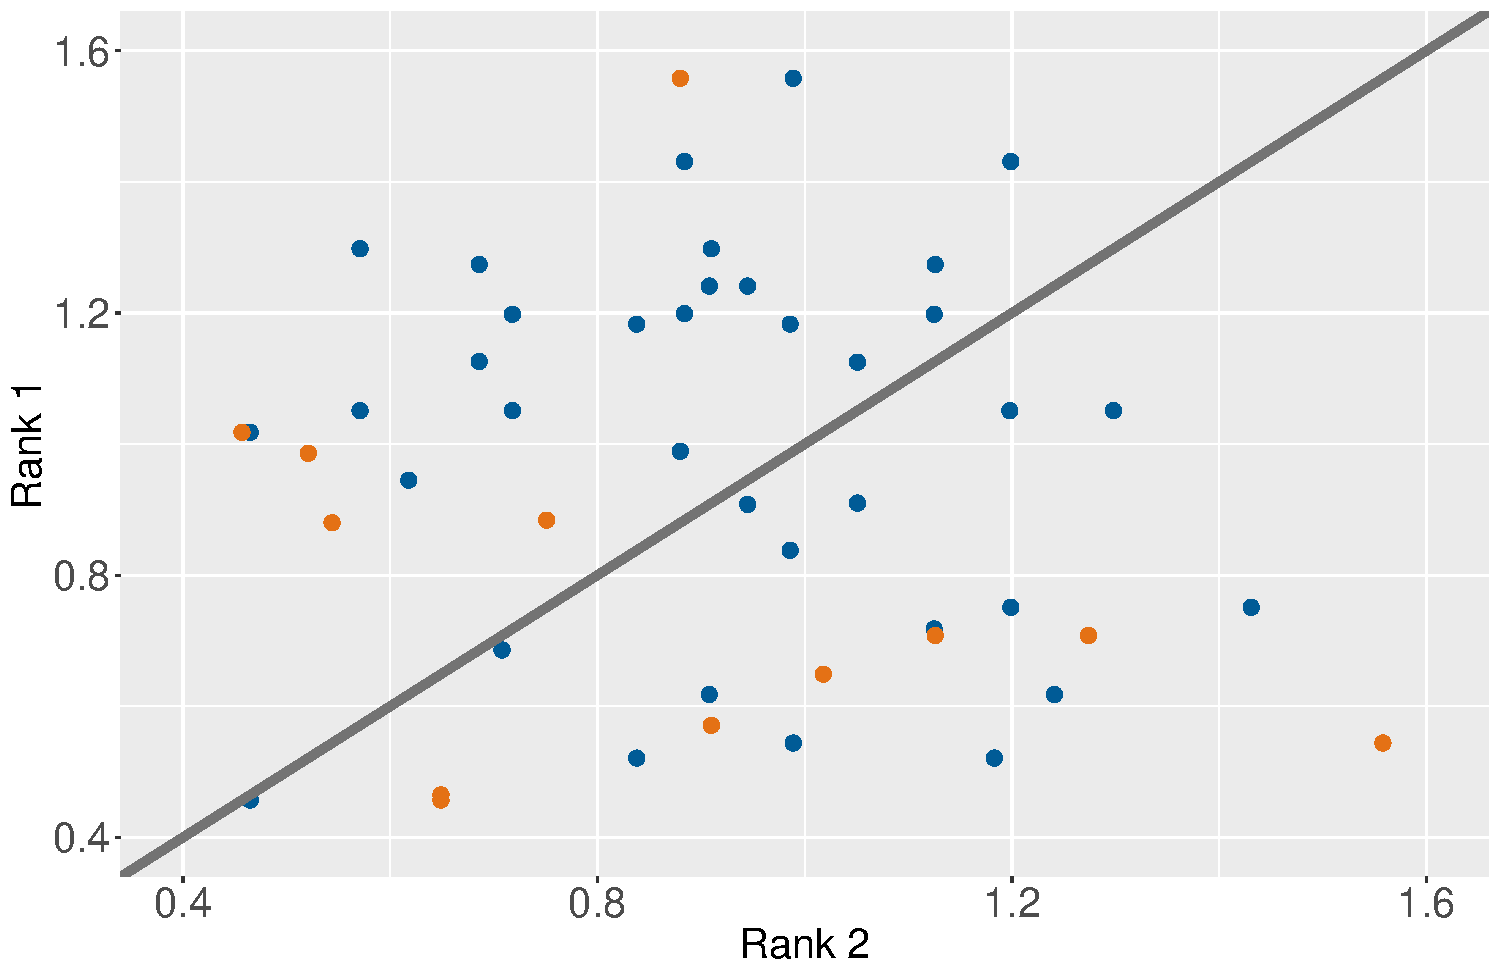
\includegraphics[scale=0.27]{ScenarioA.pdf}}~
\subfloat[Scenario B]
{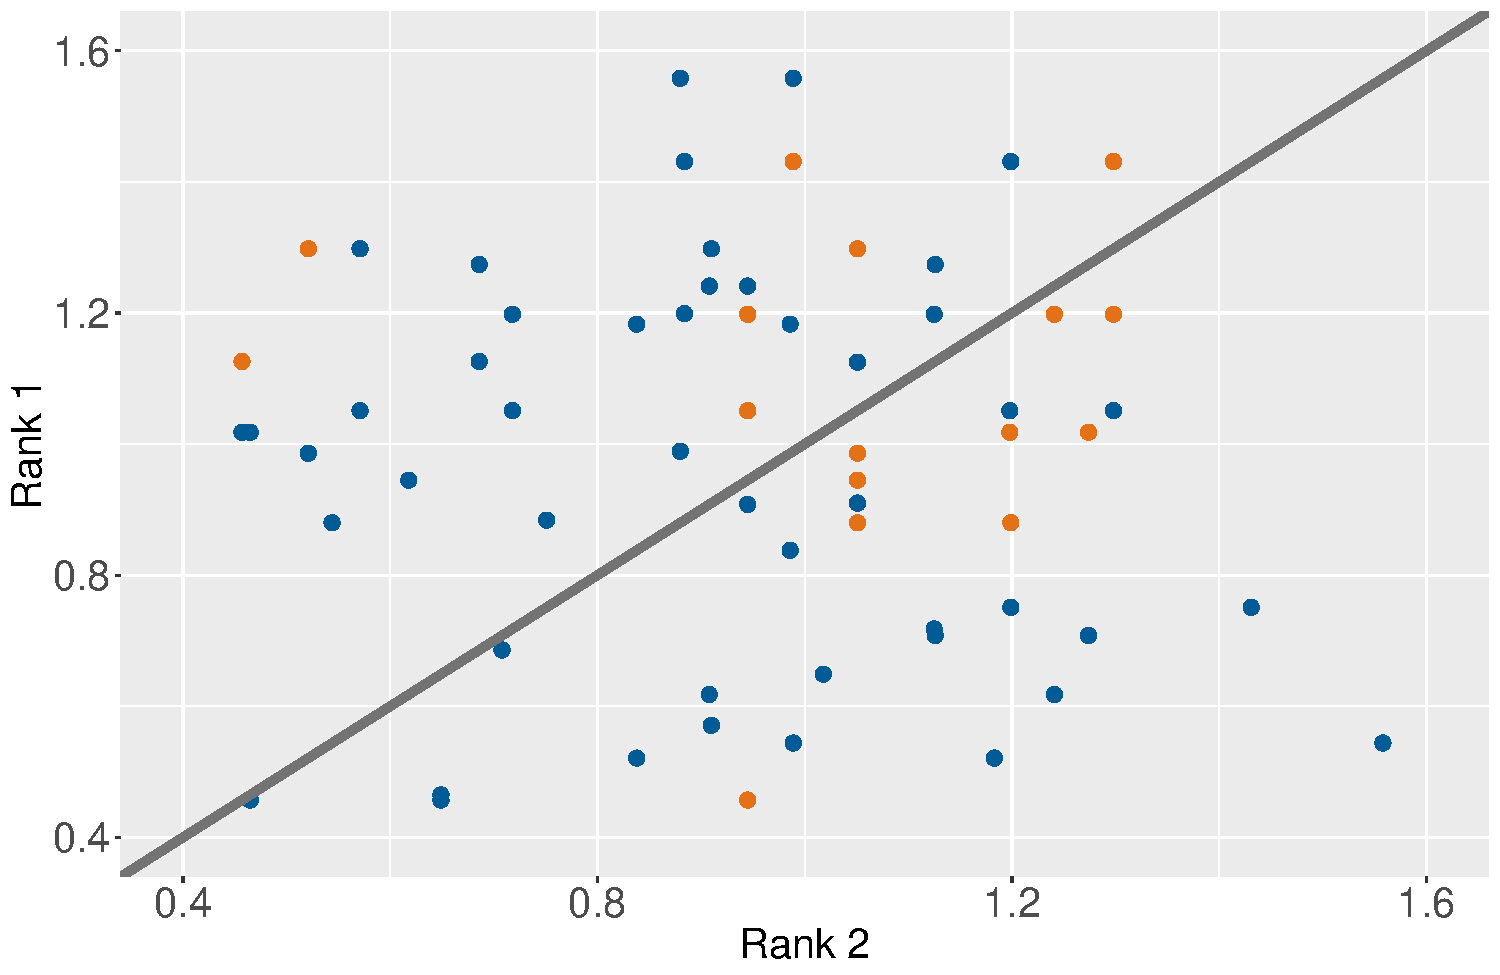
\includegraphics[scale=0.27]{ScenarioB.pdf}}\\
\centering
\subfloat[Scenario C]
{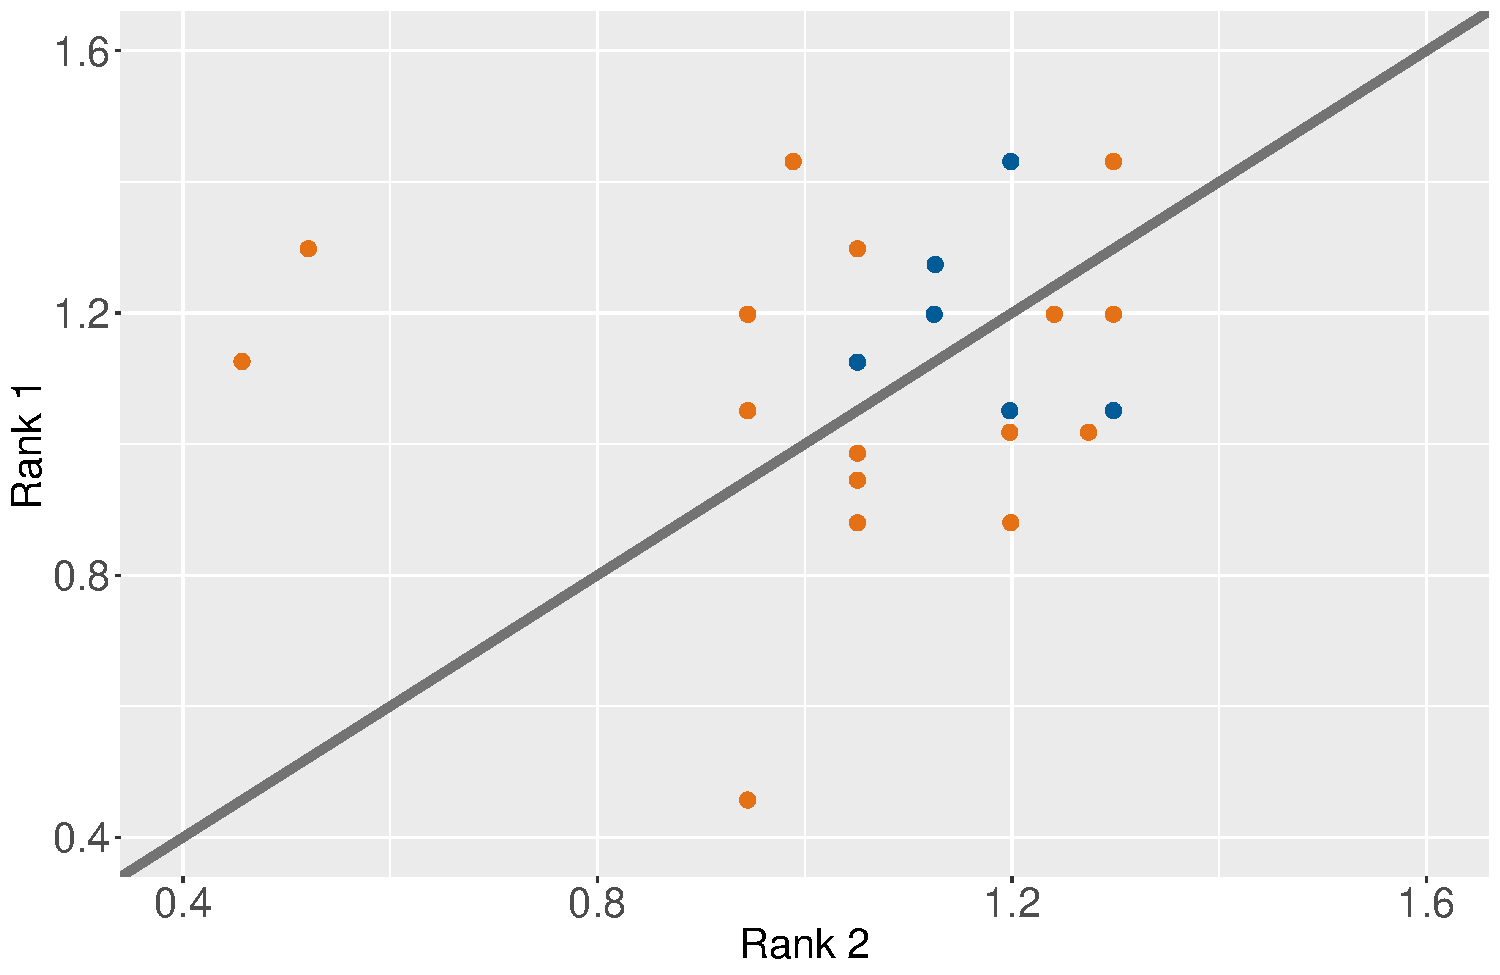
\includegraphics[scale=0.27]{ScenarioC.pdf}}
\caption{For each prediction scenarios, the values of the FIFA rankings for each match are shown in blue colour for the training set and in orange colour for the test set.}
\label{Fig1}
\end{figure}
\end{center}
%
\begin{figure}
\centering
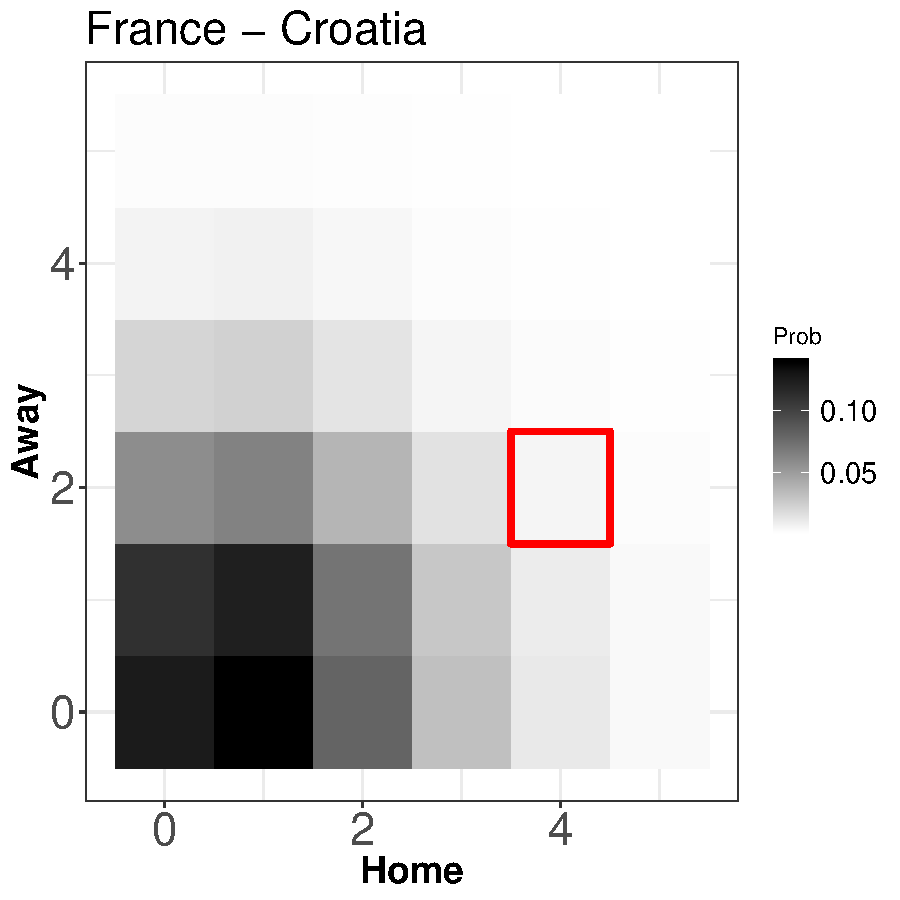
\includegraphics[scale=0.5]{France-CroatiaHeatmap_bivpois}
\caption{Posterior prediction distribution of the goals for the final France-Croatia}
\label{Fig2}
\end{figure}
%
Figure~\ref{Fig1} displays for each scenario the values for the FIFA rankings for the training set matches (blue points) and the test set matches (orange points), along with the 
line $\text{Rank }1= \text{Rank }2$, implying that the ranking difference is $w=0$. In Scenario A, the test set matches are randomly selected from the group stage, and they do not 
show any particular pattern around the line $w=0$. In scenarios B and C, test set matches belong to the knockout stage, where the teams are expected to be stronger and 
closer each other in terms of their rankings. In fact, the majority of the orange points (13 out of 16) is displayed towards the bottom right corner---higher rankings---and closer to the line $w=0$---closer strengths. Scenario B uses more and more data to predict test set results---all the 48 group stage matches---whereas Scenario C only six matches.

Figure~\ref{Fig2} depicts the posterior predictive distribution (p5 and p7) of the number of goals scored by France and Croatia during the final from the bivariate Poisson model. Darker 
regions are associated with higher probabilities, whereas the red squadre is in correspondence with the observed result, 4-2. From this plot, one could be tempted to 
conclude that the bivariate Poisson model completely failed to predict the match; however, the global probability of France win within the 90 minutes---obtained summing the single probabilities over the lower triangle of the plot---is about 42\%, against the 29\% chance of win for Croatia (p1 and p2). Fro this plot only we can acknowledge the intrinsic variability in our model predictions (p5).

To have a glimpse about statistical and ML procedures' predictive performance, Table 2 shows the accuracy in the predictions for the seven methods and the three  scenarios. Assuming that 
higher predictive accuracies should not entirely suggest the best scientific methods (p1), we analyse the performance of the methods by focusing on pro and cons. As suggested by 
Figure~\ref{Fig1}a, Scenario A is the most noisy in terms of rankings' differences, being its test set constituted by matches randomly chosen from the group stage, without any kind 
of pattern. As it is intuitive, ML techniques (Random Forest and Neural Nets), perform better, since they `shake' the training set (p8) in such a way to retrieve the highest 
predictive accuracy. The ML performances dramatically decrease in Scenario B and C, where learning from the training set should be focused on predicting the knockout stage. ML algorithms learn less and in a very random way, but it is not clear why (p10).
As already argued, the choice of the training and the test set can dramatically 
change the predictive performance of the ML algorithms, which over-perform statistical models only when considering a portion of the group stage to predict the remaining 
group stage matches. Should maybe we conclude that statistical models are better scientific tools to predict the World Cup? Not at all (p1), but we can learn from this example to improve over the next World Cups (p4).

%Although the example is quite simple and the dataset is too small to extract general conclusions, there are enough arguments to emphasize the paradoxical performance achieved by ML techniques. Their predictive accuracy is too much influenced by the training set 
%structure, making impossible to draw conclusions about their plausibility for predicting the football World Cup. 
By concluding, from this simple case-study we cannot openly 
falsify our statistical/ML techniques on the ground of future predictions. However, Poisson models seem to be less sensitive to the training set structure, and then falsifiable in a broader sense.

\begin{center}
\begin{table}
%\centering
\caption{Prediction accuracy for the selected methods, according to three prediction  scenarios.}
\begin{tabular}{|r|rrr|}
\hline 
 \emph{Train}& 75\% group  & 100\% group  & rank $>$ 1   \\ 
  \hline
\emph{Test} & 25\% group & knockout & knockout\\ 
  \hline
\emph{Random forest} & 0.67 & 0.25 & 0.44 \\ 
  \emph{Bagged CART} & 0.67 & 0.31 & 0.37  \\ 
%  bayesglm & 0.25 & 0.19 & 0.19 \\ 
  \emph{CART} & 0.58 & 0.31 & 0.19  \\ 
  \emph{MARS} & 0.58 & 0.38 & 0.49 \\ 
  \emph{NN} & 0.67 & 0.25 & 0.44  \\ 
  %Multinomial & 0.50 & 0.50 & 0.50 \\ 
  %Multinomial  & 0.42 & 0.62 & 0.62  \\ 
  \emph{Double Pois.} & 0.58 & 0.50 & 0.56  \\ 
  \emph{Biv. Pois.} & 0.58 & 0.56 & 0.56  \\ 
   \hline
\end{tabular}
%\label{tab1}
\end{table}
\end{center}
%

%Obviously it should be noted that the results presented here are only preliminary also considering the small size of the dataset here analysed. A full appreciation of the 
%different performances  is out-of the scope of the current paper and should be definitely considered for future research, also aimed  at defining a strategy for stacking models in this specific application case.

\section{Discussion}
\label{sec:concl}

Prediction is central in the progress of science and became even more relevant in statistics and data science, as the availability of new 
computational tools became common to accomodate data and predict new events. The entire field of science changed a lot over the last 
decades, new disciplines entered in the scientific gotha, and social sciences became new frontiers where predictive accuracy was strongly required. 

Natural and physical sciences progressed by means of Popper's falsificationism philosophy, whose one of the main consequences is the 
strong predictivism: scientific theories should be falsified in light of wrong predictions. Though, social sciences are not falsifiable in the 
same way: some social events---Presidential elections, football results, policies effect---are not perfectly predictable due to many reasons, such 
as data origins and unpredictable human behaviours. In this paper, we relax the assumptions behind strong instrumentalism and we provide a 
bunch of points---see Table 1---to frame statistical and machine learning techniques within the weak instrumentalist philosophy, whose main 
proposals regard algorithm's transparency and variability in the predictions.

As statisticians demanded to build good models to accomodate complex data, we feel to warn statistics and data science users about the role of prediction. Predictive accuracy is not always constitutive of scientific success: prediction is not everything, but is vidal, and it is our responsibility to choose between the gun or the bazooka.



\bibliographystyle{chicago}
\bibliography{predbib}

\end{document}